\documentclass[final,t,20pt]{beamer}
\mode<presentation>{
  \usetheme{CPTposter}
}
\usepackage{ragged2e}

% additional packages
\usepackage{listings}
\usepackage{amsmath,amsthm, amssymb, latexsym}
\usepackage{exscale}
\usepackage[orientation=portrait,size=a0]{beamerposter}
\usepackage{tikz}
\usetikzlibrary{shapes,arrows}
\usepackage{multirow}


\title{Enhancing Student Engagement with Online Annotation of Bacteriophage Genomes}
\author{\huge Eric Rasche$^{\text{1}}$, Jason Gill$^{\text{2}}$, Ryland Young$^{\text{1, 3}}$}
\institute{\large 1. Center for Phage Technology, Texas A\&M University, College Station, United States\\2. Department of Animal Science, Texas A\&M University, College Station, United States\\3. Biochemistry and Biophysics, Texas A\&M, College Station, United States}

% abbreviations
\setlength\parindent{1cm}

\begin{document}
\begin{frame}[fragile]
    \begin{columns}[t]
        \columnPadding{0.00}
        \begin{column}{.36\linewidth}
            \begin{block}{Why Undergraduate Phage Genomics?}
                \begin{itemize}
                    \item Phages are ideal--small size, high coding
                        density
                    \item Can be annotated within a single semester, by a
                        single undergraduate
                    \item Sequencing and assembly are no longer the
                        throughput-limiting step.
                    \item Great test bed for teaching bioinformatics. Many computations are extremely fast (seconds to hours), which allows for more interactive exploration.
                \end{itemize}
            \end{block}

            \begin{block}{Previous Course Iterations}
                \justifying
                Students
                \begin{itemize}
                    \item \textbf{Students hated the command line!}
                    \item They also struggled to
                        correctly copy command line statements and failed to
                        understand the relationship between their printed
                        protocols and what they were doing on the screen.
                    \item Keeping track of a huge number of files from various
                        tool outputs was tough for untrained undergraduates.
                \end{itemize}
                Staff
                \begin{itemize}
                    \item Could not keep tabs on student progress throughout the semester.
                    \item Documenting the exact command line and parameters with which students ran software was impossible (typos, websites not under our control).
                    \item Strong dependence on mutable third party services was concerning for reproducibility.
                \end{itemize}

                These issues resulted in \emph{Completely Unreproducible Annotations} and a sub-optimal experience for everyone involved.
            \end{block}

            \begin{block}{CPT Innovations}
                Galaxy
                \begin{itemize}
                    \item Allowed the switch from a variety of third party
                        websites to a local Galaxy deployment.
                    \item Galaxy provides a single interface to all software,
                        from BLAST to InterProScan to TMHMM.
                    \item Automatic tracking of user's files and tool run history.
                    \item Automatic, standardized file organisation across all students.
                    \item Perfect documentation of precise commands run.
                    \item We could non-intrusively observe student annotation
                        progress.
                \end{itemize}
                Workflows
                \begin{itemize}
                    \item Students run workflows instead of tools one-by-one.
                    \item Everyone runs identical workflows, and admins can
                        pre-configure steps, reducing user error rate.
                \end{itemize}
                Apollo
                \begin{itemize}
                    \item Students only see the most up-to-date copy, which we
                        transparently and automatically back up.
                    \item Students cannot lose files or progress. They cannot
                        accidentally switch to an old version.
                    \item Staff could non-intrusively observe student
                        annotation progress.
                    \item Unified display of outputs of very different tools.
                \end{itemize}
            \end{block}

        \end{column}
        \columnPadding{0.00}
        \begin{column}{.60\linewidth}
            \begin{block}{Galaxy \& Apollo: Automation \& Unified Results Display }
                \begin{figure}
                    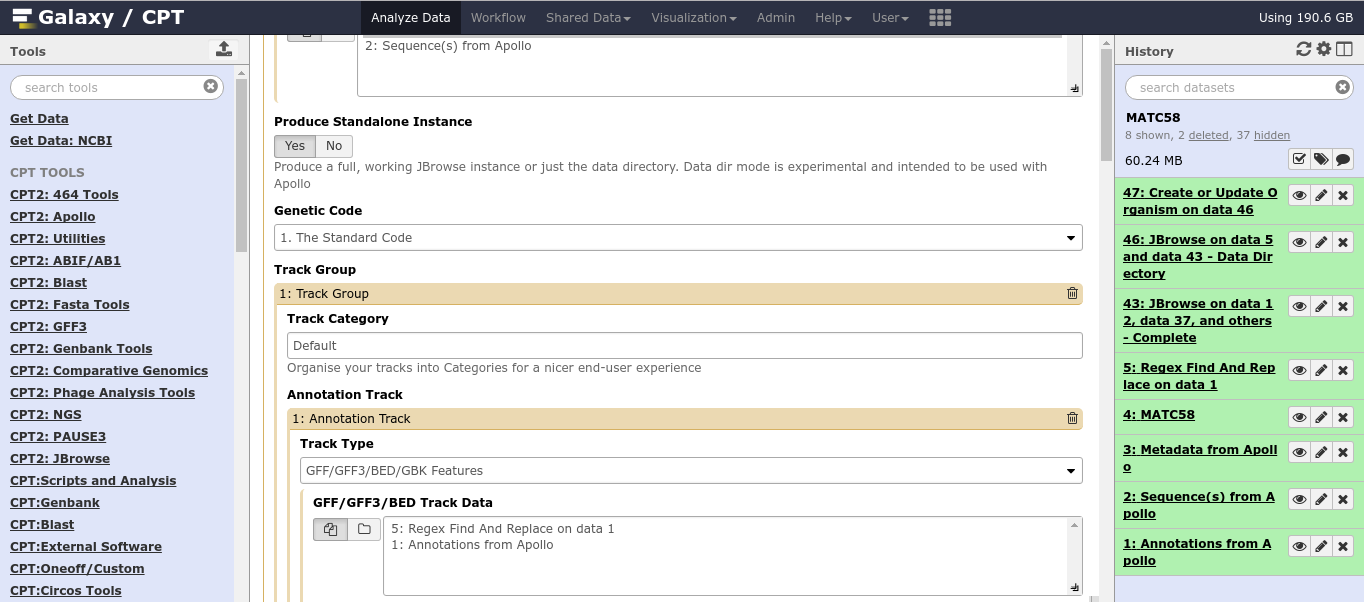
\includegraphics[width=0.98\textwidth]{./media/galaxy.png}
                    \caption{In \textbf{Galaxy}, every tool has a standardized
                        interface. Once students learn the interface, they can
                        use any of the $\approx$600 tools available in the
                        CPT's Galaxy, just by understanding the tool's use case.}
                \end{figure}
                \begin{figure}
                    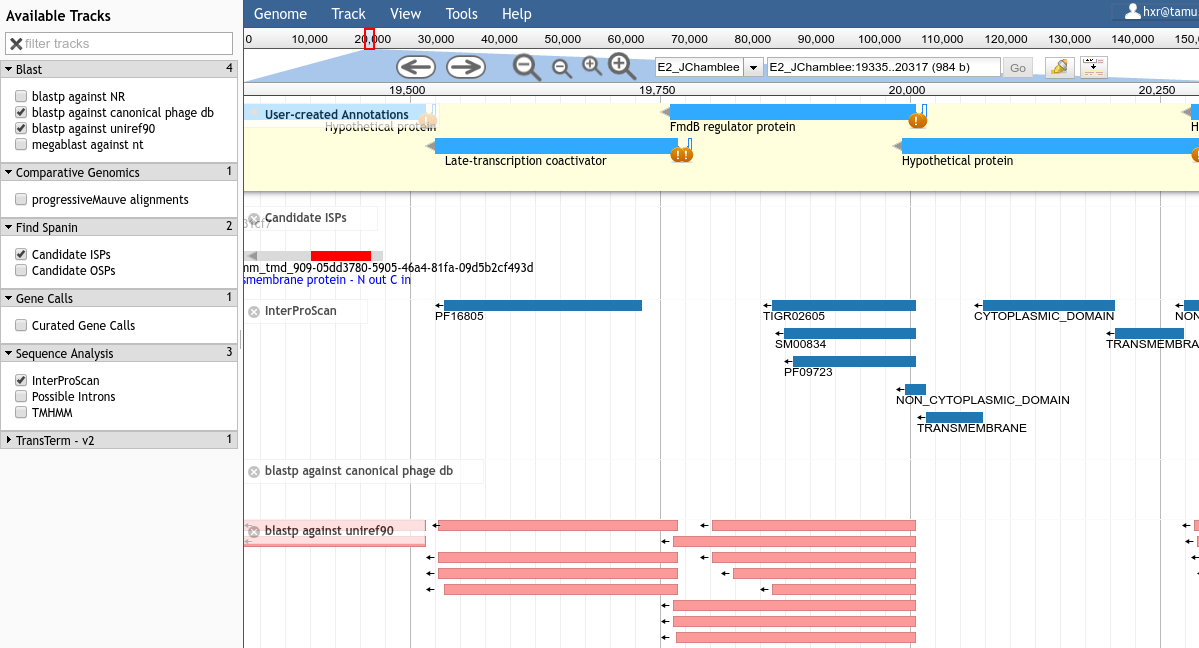
\includegraphics[width=0.98\textwidth]{./media/apollo.png}
                    \caption{\textbf{Apollo}, the online collaborative genome annotation
                    suite, has significantly increased student/staff
                    collaboration and productivity while decreasing IT burden.
                    Also visible: display of heterogeneous data within the Apollo
                    Genome Browser. Results from highly disparate HTML pages,
                    text files, etc. are visually unified, allowing researchers to
                    focus on biology.}
                \end{figure}

                \begin{figure}
                    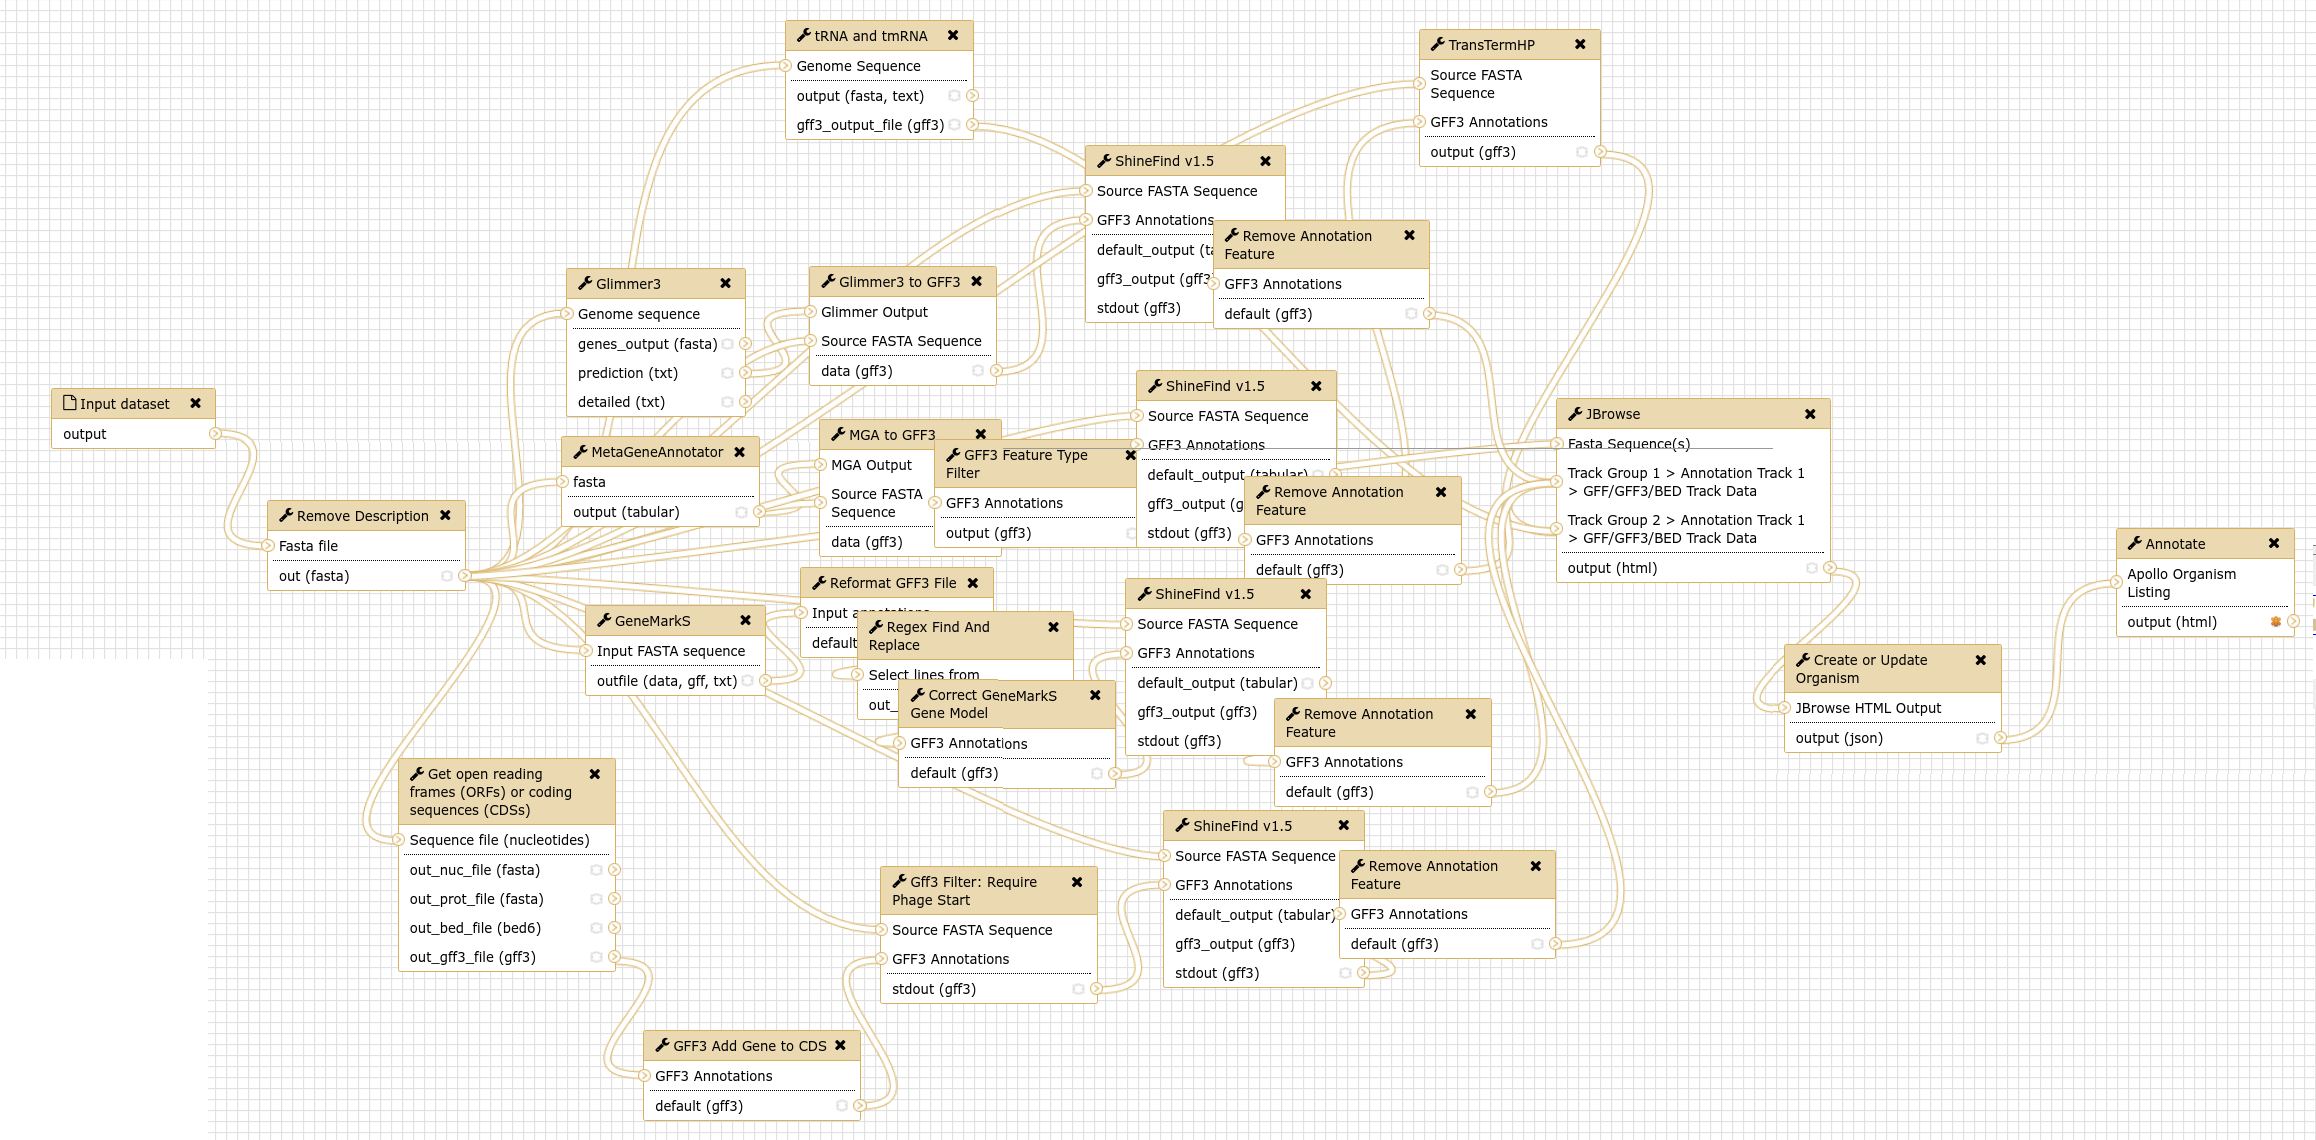
\includegraphics[width=\textwidth]{./media/workflow.png}
                    \caption{Galaxy Workflows enable researchers to develop
                    common analysis units such as ``Gene Calling'', and to
                    adjust these workflows whenever new and improved methods
                    become available. We recently added MetaGeneAnnotator to our
                    gene callers. Students and researchers could then
                    compare identically-styled GeneMarkS, Glimmer3, and MGA
                    outputs in Apollo, bypassing the opaqueness of large text
                    files, and cutting right to the biology.}
                \end{figure}
            \end{block}
        \end{column}
  \end{columns}
\end{frame}
\end{document}
